\documentclass{beamer}
\usetheme{Boadilla}

\usepackage{ngerman}				% neue deutsche Rechtschreibung
\usepackage[utf8]{inputenc} 		% Umlaute im Text
\usepackage[T1]{fontenc}
\usepackage{xspace}                 % Vermeidung von "ineinanderfallenden f's", wie z.B. bei Schifffahrt
\usepackage{url}		            % korrekte Anzeige/Umbruch von URLs
\usepackage{listings}               % z.B. nützlich zum Einbinden von Quellcode
\usepackage{hyperref} 				% für Hyperlinks in PDF-Dokumenten 
\usepackage{lmodern}
\usepackage{enumerate}
\usepackage[autostyle]{csquotes}
\usepackage{amsthm}
\usepackage{amsmath}
\usepackage{amssymb}

% Bib
\usepackage[backend=biber,style=numeric, citestyle=ieee]{biblatex}
\addbibresource{Literatur/quellen.bib} %Imports bibliography file

\nocite{arora_computational_2009}
\nocite{sipser_introduction_2012}
\nocite{rothe_komplexitatstheorie_2008}
\nocite{aaronson_scott_2016}
\nocite{goos_relativized_1986}
\nocite{rossman_complexity_2015}
\nocite{schaefer_completeness_nodate}

% Grafiken
\usepackage{graphicx} 				% Grafiken einfügen (pdf,png - aber jpg vermeiden)
\graphicspath{{./Bilder/}}          % Pfad zu den Bildern

\title{Polynomialzeithierarchie}
\subtitle{Seminar Komplexität}
\author{Edgar Wolf}
\institute{Hochschule Kempten}
\date{13.07.2022}

\AtBeginSection[]
{
  \begin{frame}
  \tableofcontents[currentsection]
  \end{frame}
}

\theoremstyle{plain}
\newtheorem{satz}{Satz}

\theoremstyle{plain}
\newtheorem{conjecture}{Vermutung}

\begin{document}

\begin{frame}
    \titlepage
\end{frame}

\begin{frame}
    \frametitle{Agenda}
    \tableofcontents
\end{frame}

\input{Kapitel/einführung.tex}
\section{Alternierung}

\begin{frame}
    \frametitle{Alternierung}
    \framesubtitle{Begriffsklärung}
    Alternierung kann als Verallgemeinerung des Nichtdeterminismus aufgefasst werden, und ist somit ebenfalls ein Konzept, dass in der Praxis kaum umzusetzen ist.
    Während beim Nichtdeterminismus nach einem akzeptierenden Berechnunspfad gesucht wird, können in der Alternierung die Berechnungen quantifiziert werden.
\end{frame}

\subsection{Begriffsklärung}
\begin{frame}
    \frametitle{Alternierung}
    \framesubtitle{Begriffsklärung}
    Die Zustände einer Berechnung einer alternierenden Berechnung sind (neben akzeptierenden und verwerfenden Zuständen) entweder:
    \begin{itemize}
        \item existenziell: Die Berechnung akzeptiert, wenn mind. eine Berechnung akzeptiert
        \item universell: Die Berechnung akzeptiert, wenn alle Berechnungen akzeptieren.
    \end{itemize}
    Bei einem nichtdeterministischen Algorithmus wird lediglich in einem existenziellen Modus operiert,
    sodass wir umgekehrt den Nichtdeterminismus als Spezialfall der Alternierung auffassen können.

\end{frame}


\begin{frame}
    \frametitle{Alternierung}
    \framesubtitle{Alternierender Berechnungsbaum \cite[S.409]{sipser_introduction_2012}}
     \begin{figure}
        \centering
        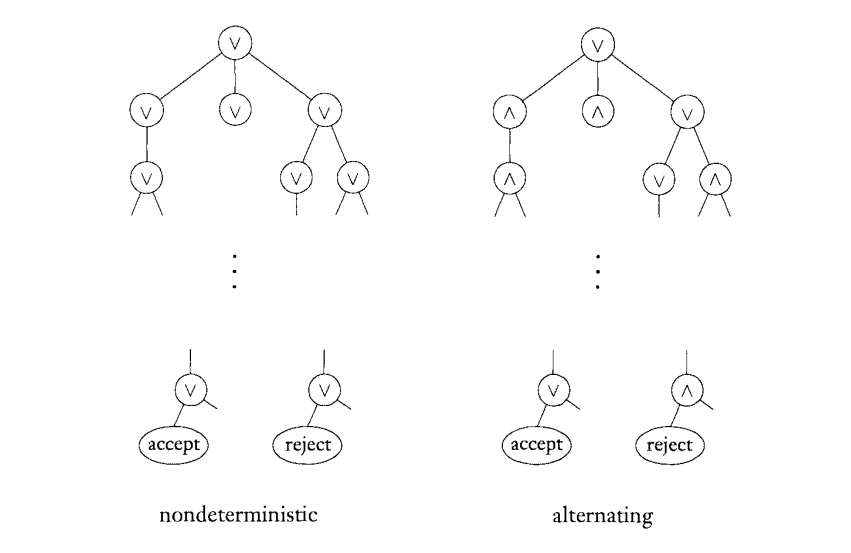
\includegraphics[scale=0.5]{Bilder/Alternierender Berechnugspfad.PNG}
        \label{Alternierende Berechung}
    \end{figure}

\end{frame}

\subsection{Alternierende Turingmaschinen}
\begin{frame}
    \frametitle{Alternierende Turingmaschinen}
    Das Konzept der Alternierung lässt sich auf Turingmaschinen anwenden. 
    Dadurch wird eine neue Klasse von Turingmaschinen definiert, die die Beschränkungen des
    Nichtdeterminismus überwinden.
\end{frame}

\begin{frame}
    \frametitle{Alternierende Turingmaschinen}
    \framesubtitle{Definition}
    \begin{block}{\textbf{Alternierende Turingmaschine}}
        Eine alternierende Turingmaschine ist eine Turingmaschine, die in einem Berechungsschritt in mehrere Zustände übergehen kann,
        und deren Zustände existenziell und universell quantifiziert werden können.
    \end{block}
    Analog zur Betrachtung des Nichtdeterminismus als Spezialfall der Alternierung kann hier eine nichtdeterministische Turingmaschine als Spezialfall einer alternierenden
    Turingmaschine betrachtet werden, die lediglich mit einem existenziellen Zustand ihre Berechnungen durchführt.

\end{frame}

\begin{frame}
    \frametitle{Alternierende Turingmaschinen}
    \framesubtitle{Akzeptanz}
    \begin{block}{\textbf{Akzeptanz einer alternierenden Turingmaschine}}
        Sei $G_{M,x}$ der Konfigurationsgraph einer alternierenden Turingmaschine $M$ auf die Eingabe $x \in \{0, 1\}^*$.
        Dann ist die Akzeptanz von $M$ auf die Eingabe $x$ über folgenden Markierungsalgorithmus definiert:
        \begin{itemize}
            \item Markiere alle Konfiguration terminierend in einem akzeptierenden Zustand $C_{accept}$ mit \texttt{ACCEPT}.
            \item Wenn eine Konfiguration $C$ mit $\exists$ markiert ist, und es eine Kante von $C$ zu $C'$ mit
            Markierung \texttt{ACCEPT} gibt, markiere $C$ mit \texttt{ACCEPT}.
            \item Wenn eine Konfiguration $C$ mit $\forall$ markiert ist, und alle Kanten von $C$ zu
            Konfigurationen $C'$ mit Markierung \texttt{ACCEPT} führen, markiere $C$ mit \texttt{ACCEPT}.
        \end{itemize}
        Die Maschine $M$ akzeptiert genau dann, wenn keine Markierung mehr möglich ist und die Startkonfiguration $C_{start}$ mit \texttt{ACCEPT}
        markiert ist.
    \end{block}

\end{frame}

\begin{frame}
    \frametitle{Alternierende Turingmaschinen}
    \framesubtitle{Alternierende Komplexitätsklassen}
    Alternierende Turingmaschinen werden bezüglich ihrer Zeit- und Platz-Beschränkung ebenso in Komplexitätsklassen unterteilt, wie 
    es für bereits für die ihre deterministischen bzw. nichtdeterministischen Äquivalente bekannt ist.
    \begin{block}{\textbf{Alternierende Komplexitätsklassen}}
        \begin{itemize}
            \item ATIME($f(n)$) ist die Menge aller Sprachen, die von einer $f(n)$-zeitbeschränkten alternierenden Turingmaschine entschieden werden können.
            \item ASPACE($f(n)$) ist die Menge aller Sprachen, die von einer $f(n)$-platzbeschränkten alternierenden Turingmaschine entschieden werden können. 
        \end{itemize}
    \end{block}
    Anhand dieser allgemeinen Definitionen können analog zu DTIME und P, oder NTIME und NP konkrete Komplexitätsklassen definiert werden.
\end{frame}

\begin{frame}
    \frametitle{Alternierende Turingmaschinen}
    \framesubtitle{Alternierende Komplexitätsklassen}
    
    \begin{block}{\textbf{Die Klasse AP}}
        AP = $\bigcup_{c \in \mathbb{N}}$ ATIME($n^c$) \\
        AP ist die Menge aller Sprachen, die von einer polynomiell zeitbeschränkten alternierenden Turingmaschine entschieden werden können.
    \end{block}

    \begin{block}{\textbf{Die Klasse APSPACE}}
        APSPACE = $\bigcup_{c \in \mathbb{N}}$ ASPACE($n^c$) \\
        APSPACE ist die Menge aller Sprachen, die von einer polynomiell platzbeschränkten alternierenden Turingmaschine entschieden werden können.
    \end{block}

\end{frame}


\begin{frame}
    \frametitle{Alternierende Turingmaschinen}
    \framesubtitle{Alternierende Komplexitätsklassen}
    
    Gerade für die Klasse AP ergibt sich dabei ein interessanter Zusammenhang zur Klasse PSPACE:

    \begin{block}{\textbf{Satz}}
        AP $=$ PSPACE
    \end{block}



\end{frame}


\begin{frame}
    \frametitle{Alternierende Turingmaschinen}
    \framesubtitle{AP $=$ PSPACE}
    
    \begin{proof}[Beweis]
        \begin{itemize}
            \item PSPACE $\subseteq$ AP: Simulation einer polynomiell platzbeschränkten TM $M$ durch eine polynomiell zeitbeschränkte ATM $M'$: $M'$ prüft die Erreichbarkeit von zwei Knoten im Konfigurationsgraph von $M$ mit einer angepassten Variante des Satz von Savitch. $M'$ rät existenziell eine Konfiguration zwischen $c_1$ und $c_2$, und prüft dann universell, ob $c_1 c_m$ in höchstens $\frac{k}{2}$ Schritten erreichen kann und selbiges für $c_m$ und $c_2$.
            \item AP $\subseteq$ PSPACE: Simulation einer polynomiell zeitbeschränkten ATM $M$ durch eine polynomiell platzbeschränkten TM $M'$: $M'$ führt eine Tiefensuche im Konfigurationsgraph von $M$ durch und bestimmt die Konfigurationen mit einem akzeptierenden Zustand. $M'$ akzeptiert, wenn ein Pfad rekonstruiert werden kann, sodass der Knoten der Startkonfiguration akzeptiert. 
        \end{itemize}
    \end{proof}
\end{frame}
\section{Defintionen der PH}
\begin{frame}
    \frametitle{Polynomialzeithierarchie}
    Die Polynomialzeithierarchie ist... 
    \begin{itemize}
        \item ein Formalismus zur Verallgemeinerung des Nichtdeterminismus
        \item eine hierarchische Struktur über polynomiell zeitbeschränkte Komplexitätsklassen
        \item ist in PSPACE enthalten
        \item ein Modell zur Beschreibung von Problemen wie z.B. \texttt{EXACT-INDSET}
    \end{itemize}
    Die Definition kann dabei über verschiedene Ansätze erfolgen.
\end{frame}

\subsection{Definition über alternierende Quantoren}
\begin{frame}
    \frametitle{Polynomialzeithierarchie}
    \framesubtitle{Definition über alternierende Quantoren}
    \begin{block}{\textbf{Definition über alternierende Quantoren}}
        Eine Sprache $L$ ist in $\Sigma^p_i$ mit $i \geq 1$ und einem Polynom $p$, wenn es eine polynomiell zeitbeschränkte Turingmaschine $M$ gibt, sodass für jede Eingabe $x \in \{0, 1\}^*$ gilt:

        \small
        \begin{align*}
            x \in L \Leftrightarrow \exists u_1 \in \{0,1\}^{p(|x|)} \forall u_2 \in \{0,1\}^{p(|x|)} ... Q_i u_i \in \{0,1\}^{p(|x|)} M(x, u_1, ..., u_i) = 1
        \end{align*}
        wobei $Q_i = \exists$ wenn $i$ ungerade ist und $Q_i = \forall $ sonst \\
       Die Definition für $\Pi^p_i$ erfolgt analog zu der $\Sigma_i^p$ mit entsprechender Quantifizierung:
        \small
        \begin{align*}
            x \in L' \Leftrightarrow \forall u_1 \in \{0,1\}^{p(|x|)} \exists u_2 \in \{0,1\}^{p(|x|)} ... Q_i u_i \in \{0,1\}^{p(|x|)} M(x, u_1, ..., u_i) = 1
        \end{align*}
        Die PH ist definiert als die Vereinigung dieser Klassen:
        \begin{align*}
            \text{PH} = \bigcup_{i \geq 1} \Sigma^p_i = \bigcup_{i \geq 1} \Pi^p_i 
        \end{align*}
    \end{block}
\end{frame}

\subsection{Definition über alternierende Turingmaschinen}
\begin{frame}
    \frametitle{Polynomialzeithierarchie}
    \framesubtitle{Definition über alternierende Turingmaschinen}
    \begin{block}{\textbf{$\Sigma_i$TIME($f(n))$}}
        $\Sigma_i$TIME$f(n)$ ist die Menge aller Sprachen, die von einer $f(n)$-zeitbeschränkten alternierenden Turingmaschine mit existenziellem Startzustand mit höchstens $i-1$ Alternierungen entschieden werden kann.
    \end{block}
    \begin{block}{\textbf{$\Pi_i$TIME($f(n)$)}}
        $\Pi_i$TIME$f(n)$ ist die Menge aller Sprachen, die von einer $f(n)$-zeitbeschränkten alternierenden Turingmaschine mit universellem Startzustand mit höchstens $i-1$ Alternierungen entschieden werden kann.
    \end{block}
    
\end{frame}

\begin{frame}
    \frametitle{Polynomialzeithierarchie}
    \framesubtitle{Definition über alternierende Turingmaschinen}
    \begin{block}{\textbf{Definition über alternierende Turingmaschinen}}
        \begin{align*}
            \Sigma^p_i = \bigcup_{c \in \mathbb{N}} \Sigma_i TIME(n^c) \\
            \Pi^p_i = \bigcup_{c \in \mathbb{N}} \Pi_i TIME(n^c) \\
            \text{PH} = \bigcup_{i \geq 1} \Sigma^p_i = \bigcup_{i \geq 1} \Pi^p_i 
        \end{align*}
    \end{block}
\end{frame}

\subsection{Definition über Turingmaschinen mit Zugriff auf Orakel}
\begin{frame}
    \frametitle{Polynomialzeithierarchie}
    \framesubtitle{Orakel}
    Eine weitere Definition bedient sich der Orakel:
    \begin{block}{\textbf{Definition über Turingmaschinen mit Zugriff auf Orakel}}
        Die Polynomialzeithierarchie ist für $i \geq 0$ definiert als:
        \begin{align*}
             & \Delta^p_0 = \Sigma^p_0 = \Pi^p_0 = \text{P} \\
             & \Delta^p_{i+1} = \text{P}^{\Sigma^p_i} \\
             &\Sigma^p_{i+1} = \text{NP}^{\Sigma^p_i} \\
             & \Pi^p_{i+1} = \text{coNP}^{\Sigma^p_i}, \Pi^p_{i+1} = \text{co}\Sigma^p_{i+1} \\
             & \text{PH} = \bigcup_{i \geq 0} \Sigma^p_i
        \end{align*}
    \end{block}
\end{frame}

\begin{frame}
    \frametitle{Polynomialzeithierarchie}
    \framesubtitle{Definition über Turingmaschinen mit Zugriff auf Orakel}
    Die Definition über Orakel betrachtet eine Stufe $0$, sowie die Klasse P, die Zugriff auf Orakel hat, während
    die anderen Definitionen ihre Definition in Stufe $1$ beginnen. Für die strukturelle Betrachtung der PH und bei der Frage des Kollapses spielen aber die Klassen der $\Delta^p_i$ eine nebensächliche Rolle.
\end{frame}


\section{Kollabieren der PH}
\begin{frame}
    \frametitle{Kollabieren der PH}
    Es wird nun auf die Möglichkeit eines Kollabierens der PH eingegangen.
    Da für die Betrachtung dieser Möglichkeit die Vollständigkeit in der PH von zentraler Bedeutung ist, wird zunächst diese formal eingeführt.
\end{frame}

\subsection{Vollständigkeit}
\begin{frame}
    \frametitle{Kollabieren der PH}
    \framesubtitle{Vollständigkeit}
    \begin{block}{\textbf{$\Sigma^p_i$-Vollständigkeit}}
        Eine Sprache $L$ ist $\Sigma^p_i$-vollständig, genau dann wenn $L \in \Sigma^p_i$ und wenn gilt:
        $$
        \forall L' \in \Sigma^p_i: L' \leq_p L
        $$
    \end{block}
    \begin{block}{\textbf{$\Pi^p_i$-Vollständigkeit}}
        Eine Sprache $L$ ist $\Pi^p_i$-vollständig, genau dann wenn $L \in \Pi^p_i$ und wenn gilt:
        $$
        \forall L' \in \Pi^p_i: L' \leq_p L
        $$
    \end{block}
    
\end{frame}

\begin{frame}
    \frametitle{Kollabieren der PH}
    \framesubtitle{Vollständigkeit}
    \begin{block}{\textbf{PH-Vollständigkeit}}
        Eine Sprache $L$ ist PH-vollständig, genau dann wenn $L \in \text{PH}$ und wenn gilt:
        $$
        \forall L' \in \text{PH}: L' \leq_p L
        $$
    \end{block}
    
    \begin{conjecture}
        Es gibt keine PH-vollständige Sprache.
    \end{conjecture}
    Die Überlegungen dahinter werden noch erläutert.
\end{frame}

\begin{frame}
    \frametitle{Kollabieren der PH}
    \framesubtitle{\textbf{TQBF}}
    
    Für die Erläuterungen der vollständigen Mengen der PH benötigen wir die Definition des Problems \textbf{TQBF}:
      \begin{block}{\textbf{\textbf{TQBF}}}

        \textbf{Eingabe:} Eine vollständig quantifizierte boolsche Formel mit boolscher Formel $\phi$ $Q_1u_1Q_2u_2...\phi(u_1, u_2, ...)$ mit $Q_i \in \{\exists, \forall\}\\ 
        \textbf{Frage:} Gibt es eine Belegung der $u_i$, sodass $Q_1u_1Q_2u_2...$\phi(u_1, u_2, ...)$ wahr ist?

    \end{block}
    
    \begin{block}{\textbf{Satz}}
        \textbf{TQBF} ist PSPACE-vollständig (ohne Beweis).
    \end{block}
    \textbf{TQBF} kann als eine Verallgemeinerung von SAT angesehen werden, sodass SAT ein Spezialfall von \textbf{TQBF} ist mit ausschließlich existenziellem Quantor.
    
\end{frame}

\begin{frame}
    \frametitle{Kollabieren der PH}
    \framesubtitle{Vollständige Mengen}
    \begin{block}{\textbf{$\Sigma_i$-SAT}}
        \textbf{Eingabe:} Eine quantifizierte boolsche Formel mit boolscher Formel $\phi$ $\exists u_1 \forall u_2...\phi(u_1, u_2, ...)$  und höchstens $i - 1$ Alternierungen der Quantoren\\ 
        \textbf{Frage:} Gibt es eine Belegung der $u_i$, sodass $\exists u_1 \forall u_2...\phi(u_1, u_2, ...)$ wahr ist?

    \end{block}
    
     \begin{block}{\textbf{$\Pi_i$-SAT}}
        \textbf{Eingabe:} Eine quantifizierte boolsche Formel mit boolscher Formel $\phi$ $\forall u_1 \exists u_2...\phi(u_1, u_2, ...)$ und höchstens $i - 1$ Alternierungen der Quantoren\\ 
        \textbf{Frage:} Gibt es eine Belegung der $u_i$, sodass $\forall u_1 \exists u_2...\phi(u_1, u_2, ...)$ wahr ist?
    \end{block}
    Diese Probleme sind $\Sigma^p_i$ bzw. $\Pi^p_i$ vollständig.
\end{frame}

\begin{frame}
    \frametitle{Kollabieren der PH}
    \framesubtitle{Vollständige Mengen}
    Ein Paper von Schafer und Umans fasst eine große Anzahl an vollständigen Problemen abseits von $\Sigma_i$-SAT und $\Pi_i$-SAT ab der Stufe $2$.
    Bekannte Beispiele sind z.B.
    \begin{itemize}
        \item \textbf{MIN DNF}
        \item \textbf{GRAPH CONSISTENCY}
    \end{itemize}
\end{frame}

\begin{frame}
    \frametitle{Kollabieren der PH}
    \framesubtitle{Vollständige Mengen}
     \begin{block}{\textbf{MIN DNF}}
        \textbf{Eingabe:} Eine boolsche Formel $\phi$ in DNF und ein $k \in \mathbb{N}$. Die Größe einer Formel sei definiert als die Anzahl der Vorkomnisse der Literale in der Formel.\\ 
        \textbf{Frage:} Gibt es eine Formel in DNF $\psi$, sodass $\psi \equiv \phi$ und die Größe von $\psi$ höchstens $k$ ist?
    \end{block}
    
    \begin{block}{\textbf{GRAPH CONSISTENCY}}
        \textbf{Eingabe:} Zwei Mengen $A$ und $B$ bestehend aus Graphen.\\ 
        \textbf{Frage:} Gibt es einen Graphen $G$, sodass jeder Graph in $A$ isomorph zu einem Teilgraphen von $G$ ist, aber kein Graph in $B$ isomorph zu einem Teilgraphen von $G$ ist?
    \end{block}
    Beide Probleme sind $\Sigma^p_2$-vollständig.
\end{frame}

\subsection{Szenarien}
\begin{frame}
    \frametitle{Kollabieren der PH}
    \framesubtitle{Kollabieren}
    Es besteht die Vermutung, dass die PH über unendlich viele Stufen verfügt, und eine Stufe als echte Teilmenge in der jeweils höheren Stufe enthalten ist. 
    Wenn die PH lediglich über eine endliche Anzahl von Stufen $k$ verfügt spricht man von einem \emph{Kollabieren} der PH auf die Stufe $k$.
    Es werden nun verschiedene Szenarien beleuchtet, die genau dazu führen würden.
\end{frame}

\begin{frame}
    \frametitle{Kollabieren der PH}
    \framesubtitle{Szenario 1: Vollständige Sprache der PH}
     \begin{block}{\textbf{Satz}}
        Sei $L$ eine PH-vollständige Sprache. Dann kollabiert die PH auf eine endliche Anzahl von Stufen.
    \end{block}
    
    \begin{proof}[Beweis]
        Da $L \in \text{PH}$ gibt es ein $i$, sodass $L \in \Sigma^p_i$.
        Außerdem gilt, da $L$ PH-vollständig ist:
        $$
            \forall L' \in \text{PH}: L' \leq_p L
        $$
        Somit können alle Problem aus den Stufen $j$ mit $j > i$ auf L reduziert werden. Das bedeutet also:
        $$
        \text{PH} \subseteq \Sigma^p_i
        $$
        Da aber jede Klasse in der PH eine Teilmenge von PH ist, folgt daraus, dass PH nur über $i$ Stufen verfügt und auf die Stufe $i$ kollabiert.
    \end{proof}
\end{frame}

\begin{frame}
    \frametitle{Kollabieren der PH}
    \framesubtitle{Szenario 2: $\Sigma^p_i = \Pi^p_i$}
     \begin{block}{\textbf{Satz}}
        Sei $i > 0$, sodass $\Sigma^p_i = \Pi^p_i$ gilt. Dann kollabiert die PH auf die Stufe $i$.
    \end{block}
    
    \begin{block}{Beweis (1).}
         Sei $L \in \Sigma^p_{i+1}$. Dann gilt:
         \small
        \begin{align*}
        x \in L \Leftrightarrow \exists u_1 \forall u_2 ... Q_{i+1}u_{i + 1} : M(x, u_1, ..., u_{i+1}) = 1
        \end{align*}
        Der Teil der Formel nach $\exists u_1$ kann dabei als Sprache $L' \in \Pi^p_i$ aufgefasst werden.
        Daraus folgt:
        \small
        \begin{align*}
        x \in L \Leftrightarrow \exists u_1 \langle x, u_1 \rangle \in L'
        \end{align*}
        Nach der Annahme, dass  $\Sigma^p_i = \Pi^p_i$ gibt ist also auch $L' \in \Sigma^p_i$, womit gilt:
        \small
        \begin{align*}
        \langle x, u_1 \rangle \in L' \Leftrightarrow \exists v_1 \forall v_2 ... Q_i v_i : M'(\langle x, u_1 \rangle, v_1, ..., v_i) = 1 
        \end{align*}
    \end{block}
\end{frame}

\begin{frame}
    \frametitle{Kollabieren der PH}
    \framesubtitle{Szenario 2: $\Sigma^p_i = \Pi^p_i$}
    
    \begin{proof}[Beweis (2)]
         Eingesetzt in die Definition der Sprache $L$ ergibt sich:
         \small
        \begin{align*}
        & x \in L \Leftrightarrow \exists u_1 \langle x, u_1 \rangle \in L' \\
        & \Leftrightarrow \exists u_1 (\exists v_1, \forall v_2, ..., Q_i v_i :  M'(\langle x, u_1 \rangle, v_1, ..., v_i) = 1) \\
        & \Leftrightarrow \exists \langle u_1, v_1 \rangle \forall v_2, ..., Q_i v_i : M'(\langle x, u_1 \rangle, v_1, ..., v_i) = 1
        \end{align*}
        Somit ist $L \in \Sigma^p_i$, wurde aber ursprünglich beliebig aus $\Sigma^p_{i+1}$ gewählt, sodass nun $\Sigma^p_i = \Sigma^p_{i+1}$ gezeigt ist. Das Kollabieren für eine Stufe $k \geq i$ auf $\Sigma^p_i$ ergibt sich induktiv:
        \begin{align*}
        \Sigma^p_{i+2} = \text{NP}^{\Sigma^p_{i+1}} = \text{NP}^{\Sigma^p_i} = \Sigma^p_{i+1} = \Sigma^p_i
        \end{align*}
    \end{proof}
\end{frame}


\begin{frame}
    \frametitle{Kollabieren der PH}
    \framesubtitle{Szenario 2: $\Sigma^p_i = \Pi^p_i$}
    Interessante Folgerungen daraus:
    \begin{itemize}
        \item Falls P = NP, dann P = PH
        \item Falls NP = coNP, dann NP = PH
    \end{itemize}
    Die Tragweite der Antworten auf diese Frage übersteigt also ihre Relation untereinander.
\end{frame}


\begin{frame}
    \frametitle{Kollabieren der PH}
    \framesubtitle{Szenario 3: PH $=$ PSPACE}
     \begin{block}{\textbf{Satz}}
        Wenn PH $=$ PSPACE, dann kollabiert die PH auf eine endliche Anzahl von Stufen. 
    \end{block}
    
    \begin{proof}[Beweis]
        \textbf{TQBF} ist bereits als PSPACE-vollständiges Problem bekannt. Da nun PH $=$ PSPACE, gibt es ein $i$ sodass \textbf{TQBF} $\in \Sigma^p_i$. Somit kann jedes $L \in \text{PH}$ auf \textbf{TQBF} reduziert werden, sodass die gesamte PH in der Stufe $i$ enthalten ist, und damit nur über $i$ Stufen verfügt.
    \end{proof}
\end{frame}


\section{Fazit}
Bla bla 

\end{document}